
\فصل{مفاهیم اولیه}

در این فصل به ذکر برخی مفاهیم اولیه‌ی مورد ارجاع در ادامه‌ی پایان‌نامه پرداخته می‌شود.
این مفاهیم در دو دسته‌ی پزشکی و فنی قابل بررسی هستند.
در ابتدا، مبانی پزشکی موضوع پروژه و نکاتی حول تصاویر پزشکی مورد استفاده به اختصار شرح داده می‌شود.
در ادامه نیز نکاتی در رابطه با هسته‌ی فنی پروژه و روش‌های مورد استفاده در یادگیری ماشین ذکر می‌گردد.
به این ترتیب، این فصل می‌تواند در دست‌یابی به یک دانش مشترک در میان متخصصان هر دو حوزه اثربخش باشد.

\قسمت{مفاهیم پزشکی}

در این قسمت ابتدا نکاتی در رابطه با سکته‌ی مغزی و انواع آن ذکر می‌شود.
سپس امتیاز ASPECT به عنوان یکی از مهم‌ترین روش‌های تشخیصی سکته و محور اصلی پروژه تعریف شده و
به نحوه‌ی تشخیص آن اشاره می‌شود.
در انتها نیز نکاتی در رابطه با تصاویر پزشکی و چالش‌های استفاده از آن‌ها در قسمت فنی مطرح می‌گردد.

\زیرقسمت{سکته‌ی مغزی}

انواع سکته‌های مغزی شامل دو دسته‌ی کلی سکته‌های 
انسدادی\footnote{Ischemic}
و 
خونریزی\footnote{Haemorrhagic} 
هستند.
سکته‌ی مغزی انسدادی به علت قطع شدن جریان خون به بخشی از مغز رخ می‌دهد که باعث از دست رفتن ناگهانی عملکرد آن ناحیه می‌شود.
در مقابل، سکته‌ی مغزی خونریزی از پاره‌شدن یک رگ خونی و یا ساختار غیر طبیعی عروقی نشأت می‌گیرد.
در یک نگاه کلی، تقریباً ۸۰٪ بیماران سکته‌ی مغزی، در دسته‌ی اول، یعنی سکته‌ی انسدادی، قرار می‌گیرند \cite{donkor2018stroke}.
این دو نوع سکته‌ی مغزی، ظاهر متفاوتی در تصاویر CT به خود می‌گیرند.
تصویر 
\ref{fig:ischemic-haemorrhagic}
 این تفاوت را نشان می‌دهد.
همانطور که در این تصویر نمایان است، عموماً تشخیص ناحیه‌ی درگیری
در سکته‌ی خونریزی ساده‌تر است و در مقابل، تشخیص این نواحی در سکته‌ی انسدادی، ظرافت و دقت بیشتری نیاز دارد.
همانطور که در تعریف امتیاز ASPECT خواهد آمد، پژوهش حاضر نیز، زیرمجموعه‌ی 
سکته‌های انسدادی قرار می‌گیرد و تمام مفاهیم مورد اشاره در این پایان‌نامه و تمام تصاویر مورد استفاده نیز به این نوع سکته اشاره خواهند داشت.

% \begin{figure}[ht]
% \centering
% 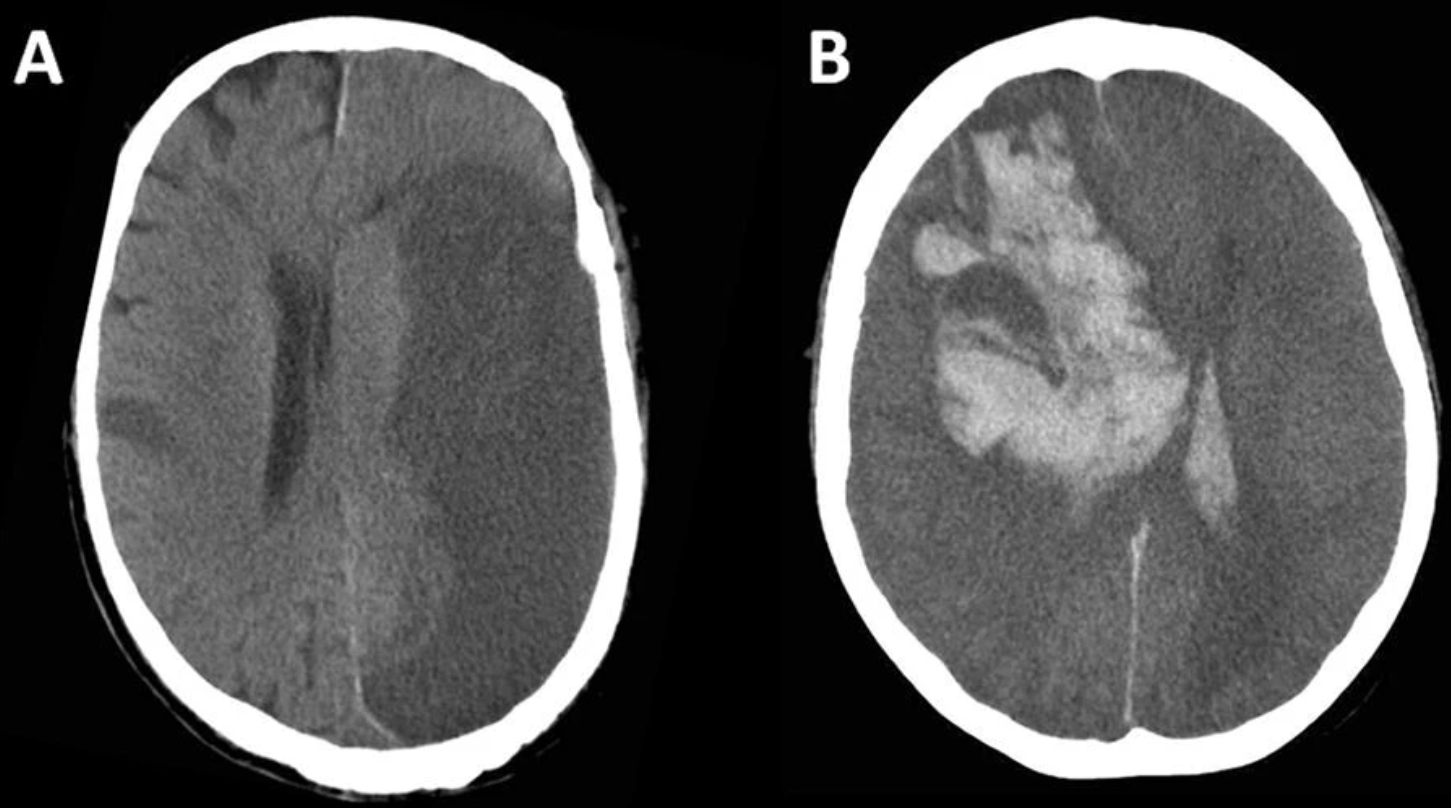
\includegraphics[width=\textwidth, keepaspectratio]{ischemic-haemorhagic.png}
% \caption[]{انواع سکته‌ی مغزی در تصاویر CT \cite{le2018ischemic}. برش مغزی A یک نمونه سکته‌ی انسدادی و برش B یک نمونه از سکته‌ی خونریزی در این تصاویر را نشان می‌دهد.}
% \label{fig:ischemic-haemorrhagic}
% \end{figure}

\شروع{شکل}[ht]
\centerimg{ischemic-haemorrhagic}{0.5\textwidth}
\caption[انواع سکته‌ی مغزی]{انواع سکته‌ی مغزی در تصاویر CT \cite{le2018ischemic}. برش مغزی A یک نمونه سکته‌ی انسدادی و برش B یک نمونه از سکته‌ی خونریزی در این تصاویر را نشان می‌دهد.}
\برچسب{fig:ischemic-haemorrhagic}
\پایان{شکل}

\زیرقسمت{امتیاز ASPECT}

ASPECTS\footnote{\lr{The Alberta Stroke Program Early CT Score}}
یک امتیاز عددی از 0 تا ۱۰ است که میزان پیشرفت تغییرات حاصل از سکته‌ی انسدادی را 
نشان می‌دهد.
 امتیاز‌دهی ،ASPECT 
 قلمرو رگ مغزی میانی در مغز را به ۱۰ ناحیه‌ی مشخص تقسیم می‌کند (تصویر ~\ref{fig:aspects-regions}).
 امتیازدهی  از ۱۰ آغاز می‌شود و به ازای هر کدام از این ۱۰ ناحیه که علائم کاهش جریان 
 خون را نشان می‌دهند، یک امتیاز از ۱۰ کم می‌شود.
 این امتیاز برای تجویز لخته‌زدایی‌های درون‌رگی و برون‌رگی برای بیماران به‌کار می‌آید \cite{mokin2017aspects}.


% \begin{figure}[ht]
% \centering
% 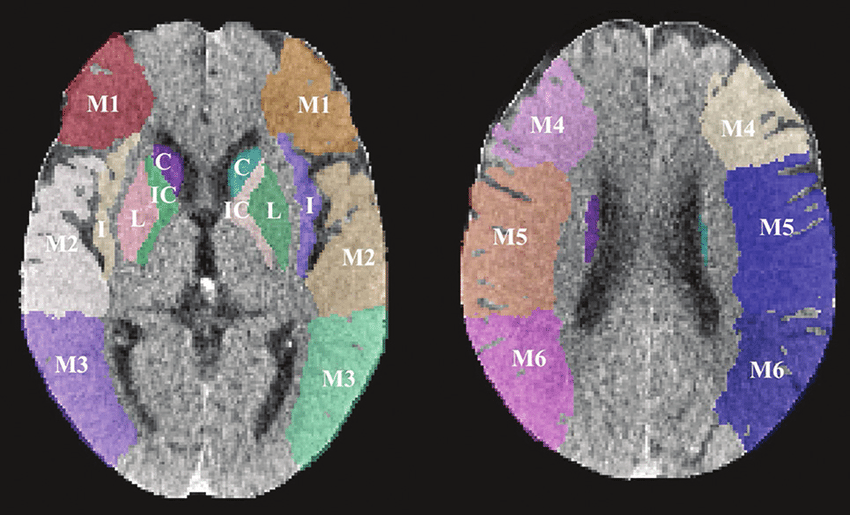
\includegraphics[width=\textwidth, keepaspectratio]{aspects-regions.png}
% \caption[]{نواحی ASPECTS در دو برش از مغز \cite{kuang2019automated}. ۱۰ ناحیه شامل ،I ،C ،L ،IC \lr{M6}-\lr{M1}.}
% \label{fig:aspects-regions}
% \end{figure}

\شروع{شکل}[ht]
\centerimg{aspects-regions}{0.7\textwidth}
\شرح[نواحی ASPECTS]{نواحی ASPECTS در دو برش از مغز \cite{kuang2019automated}. ۱۰ ناحیه شامل ،I ،C ،L ،IC \lr{M6}-\lr{M1}.}
\برچسب{fig:aspects-regions}
\پایان{شکل}

این امتیاز 
در ابتدا به این منظور طراحی شد که 
در تشخیص بیمارانی که نتایج بهتری از لخته‌زدایی درون‌رگی
کسب خواهند کرد،‌ کمک کننده باشد.
بعد‌ها از این امتیاز برای تشخیص بیمارانی استفاده شد که برای درمان لخته‌زدایی برون‌رگی مناسب نیستند.
درواقع عملیات 
باز کردن رگ‌ها\footnote{Recanalization}
در بیمارانی که علائم سکته‌ی انسدادی در نواحی وسیعی از مغزشان گسترده شده، می‌تواند بی‌اثر یا حتی زیان‌بار باشد.
اخیراً هم این امتیاز در
مجموعه‌ی دستور‌العمل‌های مدیریت سکته‌ی مغزی
انجمن قلب آمریکا به عنوان 
 یک معیار کلیدی در تجویز 
 لخته‌زدایی برون‌رگی عنوان شده‌است.
 به نحوی که این روش درمانی برای بیمارانی با امتیاز $ASPECTS\geq 6$ توصیه می‌شود \cite{mokin2017aspects}.
با این تفسیر، مشخص می‌شود علی‌رغم ۱۰ امتیازی بودن ،ASPECTS معمولاً آن‌چه که اهمیت دارد، تنها یک حد آستانه بر روی این امتیاز است.
به این نوع از امتیازدهی که وضعیت بیماران را به دو دسته‌ی بالا و پایین یک آستانه (مثلاً $ASPECTS\geq6$) تقسیم می‌کند، امتیاز 
دوبخشی‌شده‌ی\footnote{Dichotomized}
ASPECTS می‌گویند.
لازم به ذکر است که خروجی نهایی پژوهش حاصل و نتایج گزارش‌شده برای آن نیز، از نوع امتیازدهی دو‌بخشی خواهند بود.

\زیرقسمت{نحوه‌ی امتیاز‌دهی ASPECT از روی تصاویر مغزی}

همانطور که پیش‌تر ذکر شد، امتیاز ASPECTS برای یک فرد سالم برابر با ۱۰ می‌باشد و به ازای هر یک از ۱۰ ناحیه‌ی تعیین‌شده‌ای که در اثر انسداد عروقی، آسیب دیده‌باشد، یک واحد از این امتیاز کسر می‌شود تا در حادترین وضعیت به صفر برسد.
دقت داریم که هر کدام از نواحی، به صورت قرینه در دو نیم‌کره‌ی مغز وجود دارند و در هر سمتی از مغز که آسیب دیده باشند، مجموعا تنها یک امتیاز از این ۱۰ امتیاز کم می‌شود.\footnote{البته در اکثر نمونه‌های سکته‌ی مغزی انسدادی، آسیب‌دیدگی تنها در یک نیم‌کره گسترش می‌یابد.}

باید توجه داشت که هر یک از ۱۰ ناحیه‌ی ASPECTS یک حجم و ناحیه‌ی سه‌بعدی در مغز را شامل می‌شوند.
تصویر ~\ref{fig:aspects-regions} درواقع شمایی از این نواحی را تنها در برش‌های خاصی از مغز نمایش داده‌است.
این در حالی است که هر کدام از این نواحی، در چندین برش از مغز گسترده شده‌اند.
از جنبه‌ی نظری، درست آن است که در تشخیص امتیاز ،ASPECT تمام حجم مربوط به یک ناحیه درنظر گرفته‌شود.
اما در عمل، معمولاً تنها چند برش از مغز به منظور تشخیص، مورد بررسی قرار می‌گیرند.


تصویر ~\ref{fig:aspects-slices}
گستردگی نواحی ده‌گانه‌ی ASPECTS در ۸ برش مغزی را نشان می‌دهد.
اگرچه پژوهش‌هایی وجود دارند که امتیاز ASPECT را از روی تصاویر سه‌بعدی محاسبه می‌کنند اما تشخیص انسانی ASPECTS عموماً بر روی همین تعداد محدود برش انجام می‌شود.
در روش پیشنهادی این پژوهش نیز امتیازدهی ASPECT بر روی چندین برش مهم از مغز انجام می‌شود.
این در حالی است که
پژوهش‌هایی که ASPECTS را به صورت سه‌بعدی محاسبه نمی‌کنند، غالباً تنها دو برش از مغز را بررسی می‌کنند
که انطباق کمتری با روش انسانی دارد.
جزئیات این تفاوت و روش پیشنهادی این پروژه در فصل‌های آتی خواهد آمد.

% \begin{figure}[ht]
% \centering
% 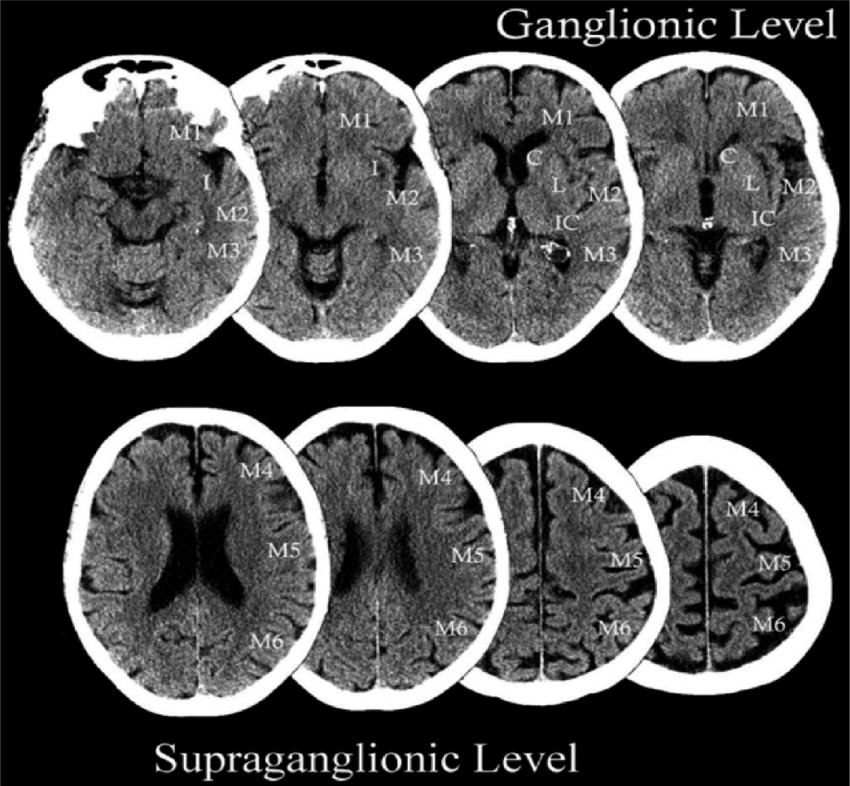
\includegraphics[width=\textwidth, keepaspectratio]{aspects-slices.png}
% \caption[]{گستردگی نواحی ده‌گانه‌ی ASPECTS در برش‌های مغز \cite{wilson2018minds}.}
% \label{fig:aspects-slices}
% \end{figure}

\شروع{شکل}[ht]
\centerimg{aspects-slices}{\textwidth}
\شرح[نواحی ASPECTS در ۸ برش مغز]{گستردگی نواحی ده‌گانه‌ی ASPECTS در برش‌های مغز \cite{wilson2018minds}}
\برچسب{fig:aspects-slices}
\پایان{شکل}

\زیرقسمت{تصاویر پزشکی}

تصاویری که در این پروژه مورد استفاده قرار گرفته‌اند، به روش\footnote{Modality}
 CT اخذ شده‌اند.
اطلاعات مربوط به هر بیمار، در قالب صدها تصویر با فرمت DICOM استخراج شده و پس از یک‌سری پردازش، برای یادگیری ماشین مورد استفاده قرار گرفته‌اند.
فرمت DICOM یک نوع فرمت مورد استفاده در تصاویر پزشکی است که علاوه بر پیکسل‌های تصویر، اطلاعاتی از قبیل نوع تصویربرداری، زمان اخذ تصویر، شناسه‌ی بیمار و \dots را در 
سرآیند\footnote{Header}
خود نگه‌داری می‌کند.
برای درک لزوم این پردازش اولیه‌ی این اطلاعات، در ادامه به برخی ویژگی‌های تصاویر پزشکی مورد استفاده به اختصار اشاره می‌شود.

\begin{enumerate}
        \item \textbf{طیف رنگی}:  چشم انسان تنها تعداد محدودی طیف رنگی خاکستری را می‌تواند تشخیص دهد. مثلاً طیف رنگی تصاویر سیاه‌سفید معمول، با اعدادی بین ۰ تا ۲۵۵ در هر پیکسل از تصویر مشخص می‌شود.
        اما تصاویر پزشکی معمولاً طیف بسیار وسیع‌تری از شدت رنگ خاکستری را شامل می‌شود. 
        ارزش هر پیکسل دراین تصاویر غالباً با واحد \lr{Hounsfield (HU)} مشخص می‌شود و عموماً می‌تواند در بازه‌ی $-1000\ HU$ تا $1000\ HU$ باشد.
        اما این طیف برای انسان قابل تشخیص نیست و باید به مقدار کمتری محدود شود تا قابل مشاهده باشد. 
         تصویر ~\ref{fig:ct-contrast-enhancement} لزوم این تغییر را نشان می‌دهد.
        \item \textbf{اضافات تصویر}: تصاویر مغزی ،CT علاوه بر بافت اصلی مغز، شامل بخش‌های دیگری هم هستند که در یادگیری و تشخیص مورد نیاز نیستند و حتی می‌توانند برای مدل ماشین، گمراه‌کننده باشند.
        از جمله‌ی این موارد، جمجمه‌ی اطراف بافت اصلی مغز، قسمت‌هایی از دستگاه تصویربرداری، هوای اطراف سر بیمار و \dots می‌باشند.
        این اضافات باید از تصویر گرفته‌شوند و تنها بافت خالص مغز برای پردازش مورد استفاده قرار بگیرند.
        \item \textbf{زاویه، محل قرار‌گیری و فاصله‌ی سر}: در حین عکس‌برداری، زاویه‌ی سر بیمار ممکن است کاملاً مستقیم نباشد.
        همچنین ممکن است سر دقیقاً در مرکز تصویر قرار نداشته باشد یا نسبت به تصویر مغز سایر بیماران، دورتر و کوچک‌تر دیده‌شود.
        این مسئله باعث تفاوت ظاهری تصاویر مغز با هم می‌شود و لازم است یک‌دست‌سازی شود.
        \item \textbf{ناحیه‌ی تصویربرداری}: در تصاویری که از مراکز مختلف تصویربرداری (و گاه از یک مرکز) جمع‌آوری می‌شوند، 
        تعداد برش‌های ثبت شده از مغز بیماران متفاوت است.
        به نحوی که در تصاویر مورد استفاده، برخی بیماران تا ۱۰ و برخی تا ۱۰۰ برش از مغز را در تصاویر خود شامل بودند.
        از طرفی همانطور که در بخش پیشین عنوان شد، تنها تعداد محدودی از برش‌های مغزی برای یادگیری و تشخیص مورد توجه هستند.
        بنابراین لازم است این برش‌های خاص، از میان ۱۰۰ ها تصویر هر بیمار جدا شوند. 
\end{enumerate}

% \begin{figure}[ht]
% \centering
% 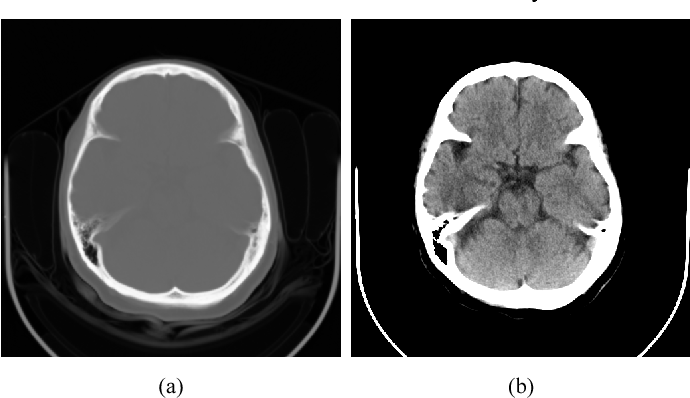
\includegraphics[width=\textwidth, keepaspectratio]{ct-contrast-enhancement.png}
% \caption[]{تفاوت توانایی تمیز جزئیات تصاویر مغز به چشم انسان، قبل و بعد از محدود کردن شدت رنگ \cite{tan2012contrast}. تصویر سمت راست، تصویر اولیه را نشان می‌دهد.}
% \label{fig:ct-contrast-enhancement}
% \end{figure}

\شروع{شکل}[ht]
\centerimg{ct-contrast-enhancement}{0.5\textwidth}
\شرح[وضوح تصاویر CT]{تفاوت توانایی تمیز جزئیات تصاویر مغز به چشم انسان، قبل و بعد از محدود کردن شدت رنگ \cite{tan2012contrast}. تصویر سمت راست، تصویر اولیه را نشان می‌دهد.}
\برچسب{fig:ct-contrast-enhancement}
\پایان{شکل}


در فصل روش پیشنهادی با جزئیات بیشتری خواهد آمد که هر یک از این چالش‌ها به چه صورت مدیریت شده‌اند و مراحل پردازش اولیه‌ی تصاویر نهایتاً به چه صورت تنظیم است.

\قسمت{مفاهیم فنی}

در این قسمت به برخی از مهم‌ترین مفاهیم یادگیری ماشین مورد استفاده در این پروژه اشاره می‌شود.
این روش‌ها به عنوان راهکاری برای مدیریت محدودیت‌های داده‌ای پروژه ارائه شده‌اند و چهارچوب کلی قسمت فنی را تشکیل می‌دهند.
جزئیات مربوط به این روش‌ها در فصل روش پیشنهادی آورده‌شده‌است.

\زیرقسمت{داده‌افزایی}

یکی از روش‌های جبران حجم کم داده‌های ورودی در یادگیری ماشین، 
داده‌افزایی\footnote{\lr{Data Augmentation}}
 است.
در این روش، با ایجاد تغییرات جزئی بر روی تصاویر ورودی، با حفظ ویژگی‌های اصلی، تعداد تصاویر افزایش داده‌می‌شود.
به عنوان مثال، با قرینه کردن تصویر مغزی که نیم‌کره‌ی راست آن درگیر است، می‌‌توان تصویر جدیدی ایجاد کرد که در آن، نیم‌کره‌ی چپ درگیر است.
هر چه که مدل ماشین، تصاویر متنوع‌تری را به این ترتیب مشاهده کند، می‌تواند بهتر بیاموزد و بر روی طیف وسیع‌تری از تصاویر، تشخیص درستی بدهد.
در پروژه‌ی حاضر نیز به منظور مدیریت تعداد محدود داده‌های ورودی، از روش‌های داده‌افزایی به خوبی بهره برده شده‌است.
با این مقدمه، در فصل روش پیشنهادی، جزئیات تغییرات اعمال‌شده بر روی تصاویر خواهد آمد.

\زیرقسمت{یادگیری انتقالی}

همانطور که مهارت و دقت متخصصان این حوزه، با کسب تجربه‌ی بیشتر، افزایش می‌یابد،
روش‌های یادگیری ماشین بر روی تصاویر نیز مبتنی بر مشاهده‌ی تعداد زیادی نمونه‌ی ورودی هستند.
البته به علت عدم هوشمندی انسانی در این مدل‌ها، نیازمندی داده‌ای به مراتب بیشتر هم هست.
هرچه تعداد نمونه‌های فراگرفته‌شده توسط مدل بیشتر باشد، دقت و عملکرد تشخیصی آن نیز بیشتر خواهد بود.
در مقابل، در صورتی که تعداد و تنوع داده‌ها اندک باشد، یادگیری ویژگی‌های کلیدی برای تشخیص، برای مدل دشوارتر خواهد بود و ممکن است تنها به حفظ‌کردن نمونه‌های مشاهده‌شده اکتفا کند.

در چنین مواردی، یکی از روش‌های مورد استفاده در حوزه‌ی یادگیری ماشین، 
یادگیری انتقالی\footnote{\lr{Transfer Learning}}
 است.
در یادگیری انتقالی، از یک مدل ماشین که توانایی‌های مشابهی با مدل مورد نیاز مسئله را دارد
استفاده می‌شود.
این مدل قبلا بر روی تعداد تعداد زیادی تصویر آموزش دیده‌است و برخی مهارت‌های پایه‌ای چون تشخیص اشیاء و مرز آن‌ها در تصاویر را فراگرفته‌است.
این مدل 
پیش‌آموزش‌دیده\footnote{Pre-trained}
سپس
به عنوان هسته‌ی مدل جدید قرار می‌گیرد تا مدل جدید بتواند از توانایی‌های آن در استخراج ویژگی‌های\footnote{Feature} تصاویر استفاده کند 
و از اطلاعاتی که این مدل به‌دست می‌دهد، برای حل مسئله‌ی خود بهره ببرد.

تعداد قابل توجهی مدل پیش‌آموزش‌دیده در حوزه‌ی یادگیری تصاویر توسعه یافته‌است.
این مدل‌ها  تا صد‌ها میلیون پارامتر یادگیری داشته و بر روی ده‌ها میلیون تصویر آموزش داده شده‌اند. 
در بخش روش پیشنهادی خواهد آمد که به‌کارگیری یادگیری انتقالی به کمک این مدل‌ها، چگونه به کاهش نیازمندی‌های داده‌ای، افزایش سرعت یادگیری و جامعیت روش پیشنهادی منجر شده‌است.

\زیرقسمت{اعتبارسنجی متقابل}

در اعتبار‌سنجی مدل‌های یادگیری ماشین، توجه به این نکته ضروری است که ارزیابی باید از روی تصاویری انجام شود که تا کنون به مدل عرضه نشده‌اند.
این تصاویر تحت عنوان داده‌های
 دیده‌نشده\footnote{Unseen}
 شناخته می‌شوند.
 درواقع
اگر مدل قبلا برچسب یک تصویر را دیده‌باشد، می‌توانسته پارامتر‌های خود را به گونه‌ای تغییر دهد که این تصویر را به درستی امتیازدهی کند.
اما آن‌چه در ارزیابی مدل، مدنظر است، توانایی مدل برای تشخیص درست بر روی تصاویر بیمارانی است که هرگز ندیده و فرانگرفته‌است.
تنها در این صورت است که می‌توان مدل را با اطمینان بالاتری در کاربرد واقعی به‌کار برد و انتظار داشت که همان عملکرد ارزیابی‌شده را بر روی داده‌های جدید از خود نشان دهد.

با این مقدمه مشخص می‌شود که
یکی دیگر از چالش‌ها در مواجهه با تعداد اندک مجموعه‌داده، در ارزیابی توانایی مدل مطرح می‌شود.
چراکه بخشی از داده‌های موجود، باید به طور کامل جدا شوند و هرگز در فرایند آموزش دخالت نداشته باشند تا سپس بتوانند در ارزیابی مدل مورد استفاده قرار بگیرند.
در این صورت، تعداد داده‌هایی که مدل می‌تواند بر روی آن‌ها آموزش ببیند، از پیش هم کمتر می‌شود.
این مسئله توانایی مدل برای یادگیری و عملکردش بر روی تصاویر دیده‌نشده را به طرز قابل توجهی کاهش می‌دهد.

شاید یک پاسخ ساده به این مشکل، این باشد که تصاویر کمتری برای ارزیابی مدل جدا شود تا مدل بتواند بر روی تعداد بیشتری تصویر آموزش ببیند.
اما این راه‌حل ممکن نیست.
زیرا عملکرد مدل بر روی تنها تعداد اندکی تصویر، نمی‌تواند ملاک مناسبی برای ارزیابی آن باشد.
این احتمال وجود دارد که مدل به صورت تصادفی، عملکرد بسیار خوبی از خود نشان بدهد.
در این صورت نتایج حاصل از ارزیابی،‌ گمراه‌کننده خواهد بود و ممکن است یک مدل نامناسب را به اشتباه وارد مرحله‌ی کاربردی کنند.

در این پژوهش، برای مقابله با این چالش از ایده‌ی روش
اعتبارسنجی متقابل\footnote{\lr{Cross Validation}}
استفاده شده‌است.
در تناظر با نام این روش، در ادامه‌ی پایان‌نامه، روش مورد استفاده برای ارزیابی مدل، ارزیابی متقابل نامیده می‌شود.
در این روش،
داده‌های موجود به ۵ دسته تقسیم می‌شوند و مدل ۵ بار وارد مرحله‌ی آموزش و ارزیابی می‌شود.
در هر مرحله، یک دسته به عنوان داده‌ی دیده‌نشده، کنار گذاشته می‌شود، مدل بر روی ۴ دسته آموزش می‌بیند و بر روی یک دسته ارزیابی می‌شود. 
به این ترتیب در طی ۵ مرحله، نهایتاً مدل بر روی تمام داده‌های موجود ارزیابی شده‌است.
زمانی که عملکرد مدل بر روی تمام داده‌های ممکن ارزیابی شد و توانایی آن قابل قبول بود، مدل بر روی تمام داده‌های موجود آموزش داده‌ می‌شود و برای کاربرد در محیط واقعی عرضه می‌شود.

به این ترتیب می‌توان گفت ارزیابی متقابل، مشکل کاهش حجم مجموعه‌داده به علت نیاز به ارزیابی مدل را حل می‌کند.
علاوه بر این، ارزیابی متقابل، روش مطمئن‌تری را برای ارزیابی مدل ارائه می‌کند.
چراکه عملکرد مدل، بر روی تمام داده‌های موجود سنجیده می‌شود و نه فقط بر روی تعدادی از تصاویر دست‌چین‌شده.
در فصل نتایج جدید مشخص می‌شود که چگونه این روش در پروژه‌ی حاضر به‌کار گرفته‌شده و به چه عملکردی منجر شده‌است.